% notes/todo

TODO: Something about the dispatchers and about what happen when things go right (near-miss)


Traditionally, safety systems are modelled as complex linear system, rather than non-linear.

\chapter{Terminology}
In general it is not recommended to say that a specific event (X) causes another (Y). This implies that X is a precondition to Y, and by eliminating X\footnote{Methods for accident investigation}

Safety: freedom from unacceptable risk

TODO: explain risk matrix

\section{Resonance}

Resonance is a phenomenon in physics making a system oscillate at a higher amplitude when a force is applied.

\section{ATC}
ATC, or Automatic Train Control

Barrier in safety engineering

general safety en resilience engineering terminology

\section{Railway}

\section{Safety systems}

\section{Classic model on safety}
%http://en.wikipedia.org/wiki/Swiss_cheese_model
Barriers are depicted as layers of swiss cheese with holes in them. 

\section{Resilience Engineering}
\label{sec:resilience_engineering}

**Stolen
The term Resilience Engineering represents a new way of thinking about safety. Whereas conventional risk management approaches are based on hindsight and emphasise error tabulation and calculation of failure probabilities, Resilience Engineering looks for ways to enhance the ability of organisations to create processes that are robust yet flexible, to monitor and revise risk models, and to use resources proactively in the face of disruptions or ongoing production and economic pressures. In Resilience Engineering failures do not stand for a breakdown or malfunctioning of normal system functions, but rather represent the converse of the adaptations necessary to cope with the real world complexity. Individuals and organisations must always adjust their performance to the current conditions; and because resources and time are finite it is inevitable that such adjustments are approximate. Success has been ascribed to the ability of groups, individuals, and organisations to anticipate the changing shape of risk before damage occurs; failure is simply the temporary or permanent absence of that.
/Stolen


\section{Human factors}
The variability of is system is becoming more and more dependent on individual and/or collective performance of humans.

Historically, this has not always been so.
TODO


\subsection{•}
**Stolen
The understanding of the human role in accidents has gone through three stages. 

In the classical view, humans were seen as error prone or as fallible machines. The purpose of an accident investigation was therefore often to find the "human error" that either was the primary (or even "root") cause or the initiating event.
When it became clear, in the 1990s, that the "human error" view was not tenable, explanations changed to look for how performance shaping factors or performance conditions could make people fail, in the sense of "forcing" errors. This did not remove the concept of a "human error", but saw these as a product of the working conditions and work pressures, rather than as a result of built-in human error tendencies.
Although this development enabled people to understand accidents of a more complex nature for a while, it still fell short in a number of situations. This led to the recognition, strongly supported by resilience engineering, that failures and successes have the same source, and that they metaphorically speaking are two sides of the same coin.
The functional resonance model (Hollnagel, 2004) describes system failure as a resonance of the normal variability of functions. To arrive at a description of functional variability and resonance, and to determine recommendations for damping unwanted variability, a FRAM analysis consists of four steps:

Identify and describe essential system functions, and characterise each function by six basic parameters.
Characterise the (context dependent) potential variability through common performance conditions.
Define the functional resonance based on possible dependencies / couplings among functions and the potential for functional variability.
Identify barriers for variability (damping factors) and specify required performance monitoring.
/Stolen
\subsection{Functional Resonance Analytic Model}

(Difference between method and model.)


\section{FRAM tools}
A special-purpose piece of computer software exists to visualize the FRAM models and conveniently describe the functions and couplings using textual input and graphical representation.

\begin{figure}[h]
 \centering
   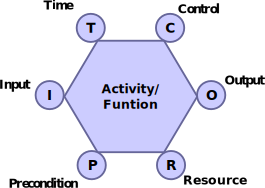
\includegraphics[width=300pt]{figures/FRAM_node.pdf}
 \caption{FRAM node}
 \label{fig:logbog}
\end{figure}
\end{document}


**Stolen
The functional resonance accident model (FRAM; Hollnagel, 2004) describes system failure
in terms of the resonance of normal performance variability. This provides a convenient way
of representing the non-linear propagation of events and also makes it possible to account for
adverse outcomes in cases where there were no manifest malfunctions or failures. The
principle of FRAM is to characterise individual system functions independently of how they
may be connected in a specific situation. The characterisation of each function ­ or node ­ is
done in terms of six aspects and the values of these aspects determine how nodes may be
coupled under given conditions. To produce a description of functional variability and
potential resonance, and to determine recommendations for damping unwanted variability, a
FRAM analysis consists of four steps:

Step 1: Identify essential system functions, and characterise each function by six basic aspects
or parameters. The six aspects are input (I, that which the function uses or transforms), output
(O, that which the function produces), preconditions (P, conditions that must be fulfilled to
perform a function), resources (R, that which the function needs or consumes), time (T, that
which affects time availability), and control (C, that which supervises or adjusts the function).
Nodes and their aspects may be described in a table and can subsequently visualized in a
hexagonal representation (cf. Figure 2 and 4 below).
Step 2: Characterize the context dependent variability of each node. For an accident analysis,
the variability is known from the investigation data. In this case the analysis focuses on
comparing the observed and the normal performance. For risk assessment, the variability may
be derived from a characterisation of the common performance conditions (CPCs), of which
there currently are eleven. These CPCs address the combined human, technological, and
organizational aspects of each function. After identifying the CPCs, the variability must be
determined in a qualitative way in terms of stability, predictability, sufficiency, and
boundaries of performance.
Step 3: Defining the functional resonance based on possible dependencies/couplings among
functions and the potential for functional variability. The output of the functional description
of step 1 is a characterisation of functions and their aspects. The aspects provides the basis for
identifying how functions may be coupled. For example, the output of one function may be an
input to another function, or produce a resource, fulfil a pre-condition, or enforce a control or
time constraint. When the couplings between functions are found, this is combined with the
characterization of performance variability from Step 2. In this way the analysis will show
how the variability of one function may have an impact on others. This analysis thus
determines how resonance, and ultimately adverse outcomes, can result from variability
across functions in the system. For example, if the output of a function is unpredictably
variable, another function that depends on this output as a resource may be performed
unpredictably. Many such occurrences and propagations of variability may have an effect like
resonance.

Step 4: Identify barriers for variability (damping factors) and specify required performance
monitoring. Barriers are hindrances that may either prevent an unwanted event from taking
place, or protect against the consequences (Hollnagel, 2004). Barriers can be described in
terms of barrier systems (the organizational and/or physical structure of the barrier) and
barrier functions (the manner by which the barrier achieves its purpose). In FRAM, four
categories of barrier systems are identified (each with their potential barrier functions, see
Hollnagel, 2004). In addition to recommendations for barriers, FRAM can also be used to
specify recommendations for the monitoring of performance and variability, as a way to
detect and manage undesired variability. Performance indicators may thus be developed for
every function and every link between functions.


\section{Retrospective FRAM}
Although FRAM is intended to be used as a design-phase tool to enhance the recilience of a system (or sub-system), its modeling characteristics enables it to be applied retrospective on an accident or near-miss event.

**Stolen
How to use FRAM for event analysis (retrospective)
An analysis using FRAM comprises the following five steps:
Define the purpose of modelling and describe the situation being analysed. Either an event that has occurred (incident/accident) or a possible future scenario (risk).
Identify the essential functions that make up the event ('foreground' functions – when things go right); characterise each by six basic aspects (Input, Output, Pre-conditions, Resources, Time, and Control). 
Characterise the actual / potential variability of 'foreground' functions and 'background' functions (context). Consider both normal and worst case variability.
Define functional resonance based on potential  / actual dependencies (couplings) among functions.
Propose ways to monitor and dampen performance variability (indicators, barriers, design / modification, etc.)
/Stolen
